\documentclass[oneside,final,14pt]{extreport}
\usepackage[utf8]{inputenc}
\usepackage[russianb]{babel}
\usepackage{vmargin}
\usepackage{amsmath}
\usepackage{amssymb}
\usepackage{amsfonts}
\usepackage{setspace}
\usepackage{indentfirst}
\usepackage{graphicx}
\setpapersize{A4}
\setmarginsrb{20mm}{20mm}{15mm}{20mm}{0pt}{0mm}{0pt}{13mm}
\onehalfspacing
\sloppy
\DeclareGraphicsExtensions{.pdf,.png,.jpg,.eps}
\newcommand\No{{\itshape N\textsuperscript{o}}}
\begin{document}
\thispagestyle{empty}
\begin{figure}[t]
  \centering
  
\includegraphics[width=0.5\textwidth]{msu}
\end{figure}
\centerline{Московский государственный университет имени М.В. Ломоносова}
\centerline{Факультет вычислительной математики и кибернетики}
\centerline{\hfill\hrulefill\hrulefill\hfill}
\vfill
\vfill
\large
\centerline{Суперкомпьютерное моделирование и технологии}
\vfill
\Large
\begin{centering}
{\bf Отчет по заданию \No 2 \\
"<Задача Дирихле для уравнения Пуассона \\
в криволинейной области">\\}
\end{centering}
\normalsize
\vfill
\centerline{ВАРИАНТ 9}
\vfill
\vfill
\vfill
\begin{flushright}
\textbf{Отчет выполнил:}\\
студент 614 группы\\
Артамонов Георгий
\end{flushright}
\vfill
\vfill
\centerline{Москва, 2023}
\newpage
\tableofcontents
\newpage
\chapter{Задача Дирихле для уравнения Пуассона}
\section{Математическая постановка задачи}
\noindent
В области \( D \subset \mathbb{R}^2 \), ограниченной контуром \(\gamma\),
рассматривается дифференциальное уравнение Пуассона (1):
\[
-\Delta u = f(x, y)
\]
в котором оператор Лапласа
\[
\Delta u = \frac{\partial^2 u}{\partial x^2} + \frac{\partial^2 u}{\partial y^2}
\]
Для выделения единственного решения уравнение дополняется
граничным условием Дирихле (2):
\[ u(x, y) = 0, \; (x, y) \in \gamma \]
Требуется найти функцию \( u(x, y) \), удовлетворяющую уравнению (1)
в области \( D \) и краевому условию (2) на ее границе. \\
Рассмотрим задачу в случае, когда правая часть уравнения \( f(x, y) = 1 \),
а область \( D \) представляет собой внутренность эллипса:
\( D = \{ (x, y) \; | \; x^2 + 4 y^2 < 1 \} \)
\section{Численный метод решения}
\subsection{Метод фиктивных областей}
\noindent
Для решения поставленной задачи предлагается использовать метод
фиктивных областей. Идея метода заключается в приближенной замене
исходной задачи Дирихле в криволинейной области
задачей Дирихле в прямоугольнике с кусочно-постоянным коэффициентом
\( k(x, y) \). Пусть область \( D \) принадлежит прямоугольнику
\( \Pi = \{(x,y) \; | \; A_1 < x < B_1, A_2 < y < B_2 \} \). Разность
множеств \( \Pi \) и \( \bar D \) обозначим \( \hat D = \Pi \setminus \bar D \),
границу прямоугольника \( \Pi \) обозначим \( \Gamma \).
\\В прямоугольнике \( \Pi \) рассмотрим задачу Дирихле (3):
\[ \begin{aligned}
  & -\frac{\partial}{\partial x}(k(x,y)\frac{\partial v}{\partial x})
  - \frac{\partial}{\partial y}(k(x,y)\frac{\partial v}{\partial y}) = F(x,y)\\
  & v(x, y) = 0, (x, y) \in \Gamma
\end{aligned} \]
с кусочно-постоянным коэффициентом:
\[ k(x, y) = 
\begin{cases}
    1,   & (x, y) \in D, \\
    1 / \varepsilon & (x, y) \in \hat D
\end{cases} \]
и правой частью:
\[ F(x, y) = 
\begin{cases}
    f(x, y),   & (x, y) \in D, \\
    0, & (x, y) \in \hat D
\end{cases} \]

Требуется найти непрерывную в \( \bar \Pi \) функцию \( v(x, y) \),
удовлетворяющую дифференциальному уравнению всюду в \( \Pi \setminus \gamma \),
равную нулю на границе \( \Gamma \) прямоугольника, и такую, чтобы вектор
потока:
\[ W(x, y) = -k(x, y)
    (\frac{\partial v}{\partial x}, \frac{\partial v}{\partial y})
\]
имел непрерывную нормальную компоненту на общей части криволинейной границы
области \( D \) и прямоугольника \( \Pi \). \\
Переход к новой задаче позволяет получить решение исходной задачи
с любой наперед заданной точностью \( \varepsilon > 0 \), решая при этом
задачу Дирихле в прямоугольнике \( \Pi \), содержащем исходную область.
\[ \max_{P \in \bar D} \|v(x, y) - u(x, y) \| \le C \varepsilon, C > 0 \]
Для случая, когда область \( D \) представляет собой внутренность эллипса,
выберем прямоугольник
\( \Pi = \{(x,y) \; | \; -1.0 < x < 1.0, -0.5 < y < 0.5 \} \).

\subsection{Разностная схема решения}
\noindent
В замыкании прямогольника \( \bar \Pi \) определим равномерную
прямоугольную сетку \( \bar \omega_h = \bar \omega_1 \times \bar \omega_2 \),
где
\[ \begin{aligned}
& \bar \omega_1 = \{x_i = A_1 + ih_1, i = 0, \ldots, M\}, \;
& h_1 = (B_1 - A_1) / M \\
& \bar \omega_2 = \{y_j = A_2 + jh_2, j = 0, \ldots, N\}, \;
& h_2 = (B_2 - A_2) / N 
\end{aligned} \]
Множество внутренних узлов сетки \( \bar \omega_h \) обозначим \( \omega_h \).\\
Рассмотрим линейное пространство \( H \) функций, заданных на сетке
\( \omega_h \).\\
Обозначим через \( w_{ij} \) значение сеточной функции \( H \) в узле сетки
\( (x_i, y_j) \in \omega_h \).
Определим скалярное произведение и норму в пространстве сеточных функций
\( H \):
\[ (u, v) = \sum_{i = 1}^{M-1} \sum_{j = 1}^{N-1} h_1 h_2 u_{ij} v_{ij} \]
\[ \| u \| = \sqrt{(u, u)} \]
Будем использовать метод конечных разностей, который заключается в замене
дифференциальной задачи математической физики на 
конечно-разностную операторную задачу вида:
\[ A \, \omega = B \]
\[ A: H \rightarrow  H \]
Дифференциальное уравнение задачи (3) во всех внутренних точках
сетки аппроксимируется разностным уравнением:
\[ \begin{aligned}
  & -\frac{1}{h_1}(a_{i+1 j} \frac{\omega_{i+1 j} - \omega_{ij}}{h_1}
- a_{ij} \frac{\omega_{ij} - \omega_{i-1 j}}{h_1})
    -\frac{1}{h_2}(b_{i j+1} \frac{\omega_{i j+1} - \omega_{ij}}{h_2}
- b_{ij} \frac{\omega_{ij} - \omega_{i j-1}}{h_2}) = F_{ij} \\
  & i = 1, \ldots, M-1, \: j = 1, \ldots, N-1
\end{aligned} \]
в котором коэффициенты при \( i = 1, \ldots, M, \: j = 1, \ldots, N \)\\
\[ a_{ij} = \frac{1}{h_2} \int_{y_{j-1/2}}^{y_{j+1/2}} k(x_{i-1/2}, t) \,dt \]
\[ b_{ij} = \frac{1}{h_1} \int_{x_{i-1/2}}^{x_{i+1/2}} k(t, y_{j-1/2}) \,dt \]
и правая часть при \( i = 1, \ldots, M-1, \: j = 1, \ldots, N-1\)\\
\[ F_{ij} = \frac{1}{h_1 h_2} \iint_{\Pi_{ij}} F(x, y) \, dx dy \]
\[ \Pi_{ij} =
\{ (x, y): x_{i-1/2} \le x \le x_{i+1/2}, y_{j-1/2} \le y \le y_{j+1/2}\} \]
Краевые условия Дирихле в задаче (3) аппроксимируются точно равенством
\[ w_{ij} = w(x_i, y_j ) = 0, \; (x_i, y_j ) \in \Gamma \]
Полуцелые узлы означают:
\[ x_{i \pm 1/2} = x_i \pm 0.5h_1, \; y_{j \pm 1/2} = y_j \pm 0.5h_2 \]
Полученная система является линейной относительно неизвестных величин
и может быть представлена в виде \( A \, \omega = B \)
c самосопряженным и положительно определенным оператором \( A \).
Построенная разностная схема линейна и имеет
единственное решение при любой правой части.\\
\noindent
Интегралы \( a_{ij}, b_{ij} \) будем вычислять аналитически:
\( a_{ij} = h_2^{-1} l_{ij} + (1 - h_2^{-1} l_{ij}) / \varepsilon \),
где \( l_{ij} \) длина части отрезка \( [y_{j-1/2}, y_{j+1/2}] \), которая
принадлежит области \( D \).
Для вычисления \( l_{ij} \) для заданного \( \hat x = x_{i-1/2} \)
вычислим точки пересечения прямой \( x = \hat x \) с границей 
эллипса \( \gamma \). Тогда \( l_{ij} = \min(y_1, y_{j+1/2}) - \max(y_2, y_{j-1/2}) \), где
\[ y_{1,2} = \pm \frac{1}{4}\sqrt{1 - \hat x^2} \]
Правую часть разностной схемы приближенно заменим на значение
в центре квадрата \( \Pi_{ij} \): 
\[ F_{ij} = F(x_i,y_j) =  \begin{cases}
    1,   & (x_i, y_j) \in D, \\
    0,   & (x_i, y_j) \in \hat D
\end{cases} \]
\subsection{Метод минимальных невязок}
\noindent
Приближенное решение разностной схемы предлагается вычислять методом
наименьших невязок.
Метод позволяет получить последовательность сеточных функций
\( \omega^{(k)} \in H, \, k = 1,2,\ldots \), сходяющуюся по норме пространства
\( H \) к решению разностной схемы.
\[ \| \omega - \omega^{(k)} \|_E \rightarrow 0, \, k \rightarrow \infty \]
Начальное приближение \( \omega^{(0)} \) выберем равным нулю во всех
точках сетки. Итерация \( \omega^{(k+1)} \) вычисляется по итерации
\( \omega^{(k)} \) по формуле:
\[ \omega_{ij}^{(k+1)} = \omega_{ij}^{(k)} - \tau_{k+1} r_{ij}^{(k)} \]
где невязка \( r^{(k)} = A \omega^{(k)} - B \), итерационный параметр
\[ \tau_{k+1} = \frac{(A r^{(k)}, r^{(k)})}{\|A r^{(k)}\|^2_E} \]
В качестве критерия останова можно использовать условие:
\[ \| r^{(k)} \|_E < \delta \]
c некоторой положительной константой \( \delta > 0 \), задающей точность
приближенного решения.
\newpage
\section{Описание программной реализации}
\noindent
Для выполнения задания был разработан последовательный код, представляющий
собой программу на языке C sequantial.c, реализующую описанный численный метод.
Были выполнены расчеты на сгущающихся сетках
\( (M, N) = (10, 10), (20, 20), (40, 40) \) и построены графики
полученных приближенных решений.
Для написания parallel.c вложенные циклы в функциях,
вызывающихся на каждой итерации метода минимальных
невязок (scalar\_product, apply\_diff\_operator, linear\_comb), были
размечены с помощью директивы OpenMP: pragma omp parallel for collapse(2). 
Были проведены расчеты на сетках (40, 40), (80, 80), (160, 160) на разном
числе потоков. Полученные приближенные решения совпали с соответствующими
решениями при последовательных вычислениях, но время их вычисления удалось
уменьшить за счет использования параллелизма. Результаты приведены в таблице.
\subsection{Результаты расчетов}
\noindent
\begin{table}[ht]
\begin{tabular}{|c|c|c|c|}
\hline
Число OpenMP-нитей & Число точек сетки \(M \times N\) &
Время решения & Ускорение \\
\hline
2  & 40 \(\times\) 40 & 91.549 & 1.298 \\
4  & 40 \(\times\) 40 & 57.722 & 2.059 \\
6  & 40 \(\times\) 40 & 48.929 & 2.430 \\
8  & 40 \(\times\) 40 & 45.768 & 2.597 \\
16 & 40 \(\times\) 40 & 46.381 & 2.563 \\
\hline
2  & 80 \(\times\) 80 & 337.001 & 1.599 \\
4  & 80 \(\times\) 80 & 183.397 & 2.938 \\
6  & 80 \(\times\) 80 & 130.966 & 4.106 \\
8  & 80 \(\times\) 80 & 111.136 & 4.848 \\
16 & 80 \(\times\) 80 & 90.581  & 5.948 \\
\hline
2  & 160 \(\times\) 160 & 321.049 & 1.689  \\
4  & 160 \(\times\) 160 & 164.734 & 3.292  \\
8  & 160 \(\times\) 160 & 86.978  & 6.235  \\
16 & 160 \(\times\) 160 & 53.271  & 10.180 \\
32 & 160 \(\times\) 160 & 51.108  & 10.611 \\
\hline
\end{tabular}
\caption{Зависимость времени решения от числа нитей для разных сеток}
\label{tab1}
\end{table}

\newpage
\subsection{Графики ускорений}
\begin{figure}[ht!]
  \centering
  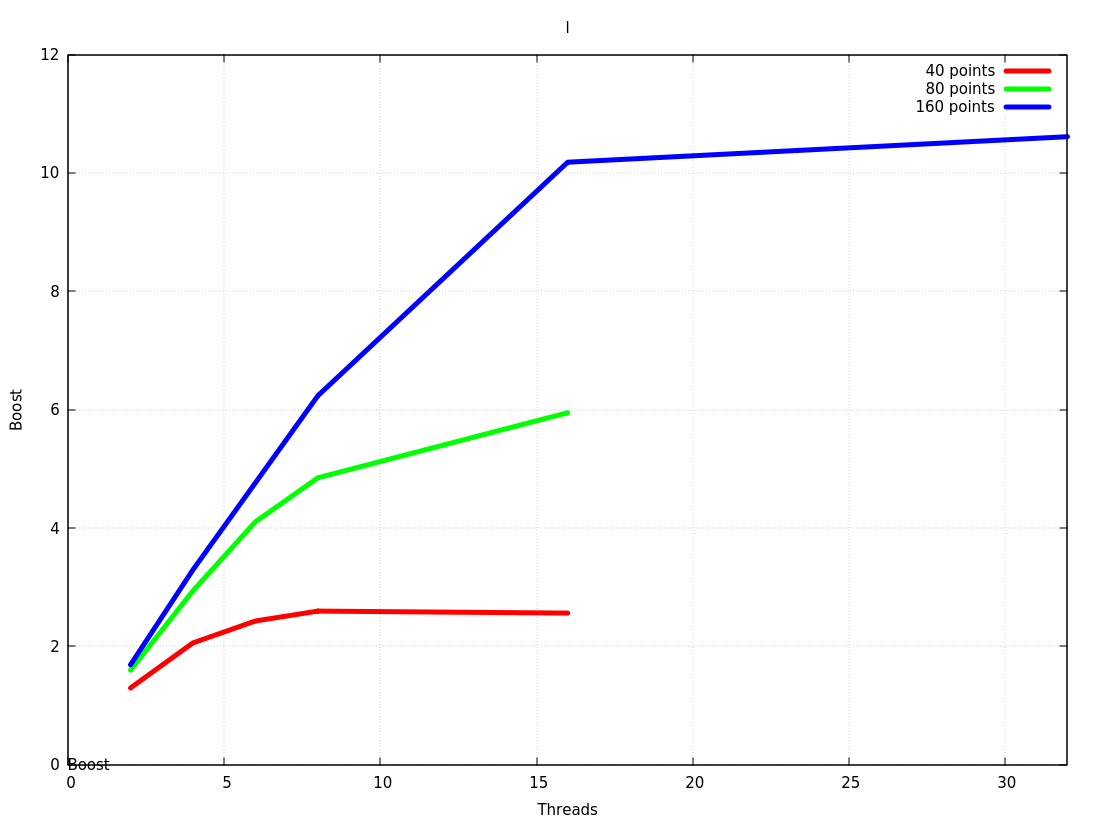
\includegraphics[width=1.0\textwidth]{picture5}
  \caption{Зависимость ускорения от числа потоков для разных для сеток}
\end{figure}

\newpage
\subsection{Графики нормы невязки}
\begin{figure}[ht!]
  \centering
  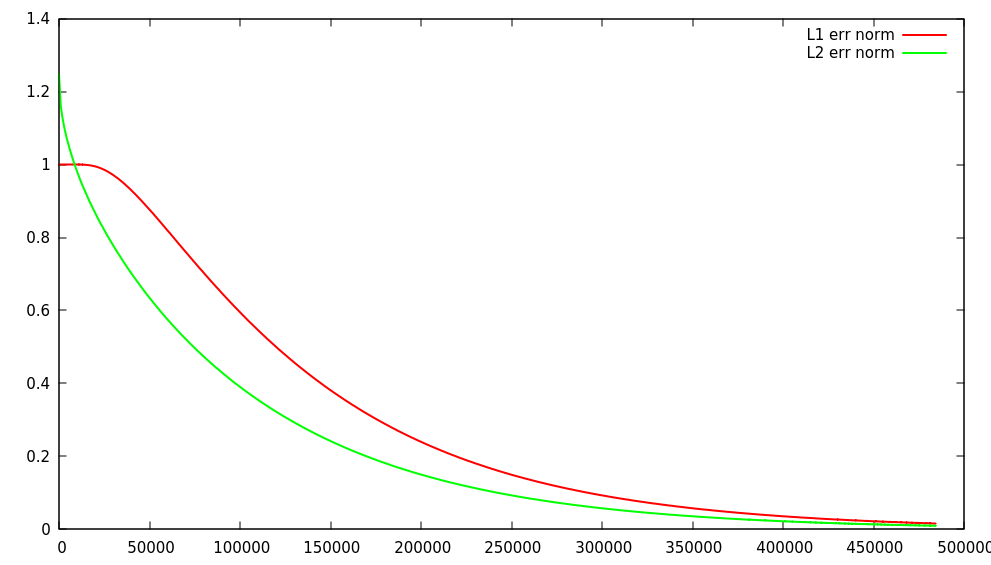
\includegraphics[width=0.9\textwidth]{picture6}
  \caption{Зависимость нормы невязки от числа итераций для сетки \((40, 40)\)}
\end{figure}

\begin{figure}[h!]
  \centering
  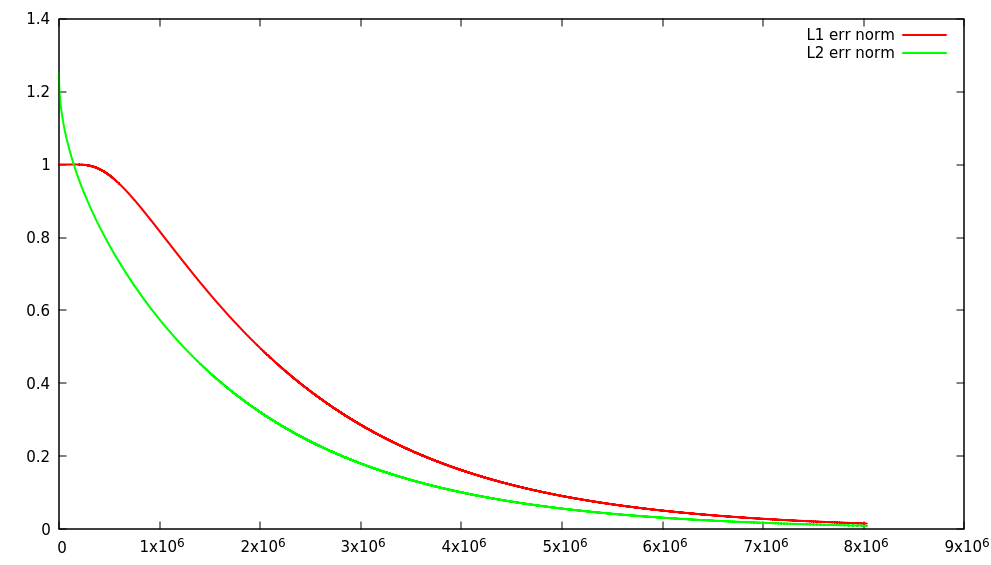
\includegraphics[width=0.9\textwidth]{picture7}
  \caption{Зависимость нормы невязки от числа итераций для сетки \((80, 80)\)}
\end{figure}

\newpage
\subsection{Точка максимума невязки}
\noindent
Построим графики для определения точек, где ошибка принимает наибольшие
значения. Каждую 1000 итераций вычисляем, в какой точке абсолютная
величина ошибки равна L1 норме невязки, иными словами, в какой точке
на этой итерации абсолютная величина ошибки принимает наибольшее значение.
Из графиков видно, что это точка \((0,0)\), являющаяся центром эллипса.
\begin{figure}[ht!]
  \centering
  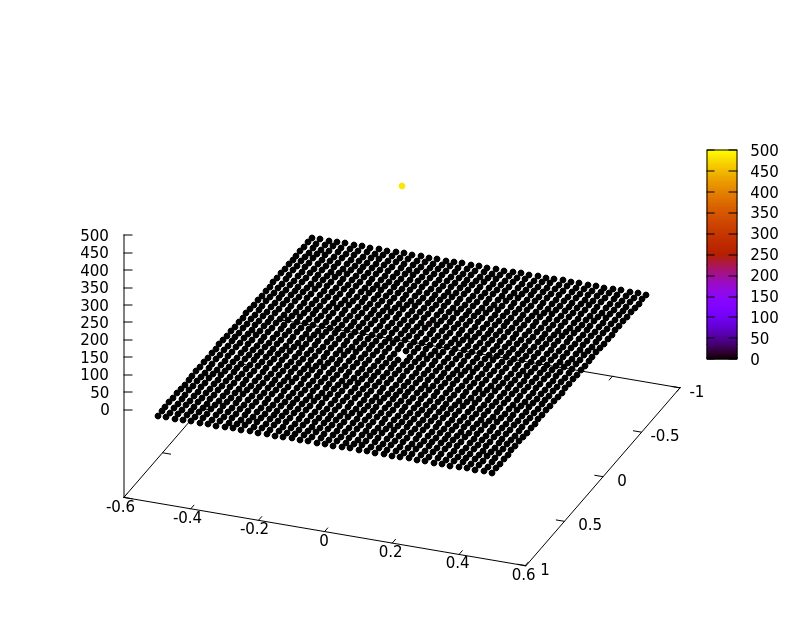
\includegraphics[width=0.6\textwidth]{picture8}
  \caption{для сетки \((40, 40)\)}
\end{figure}

\begin{figure}[h!]
  \centering
  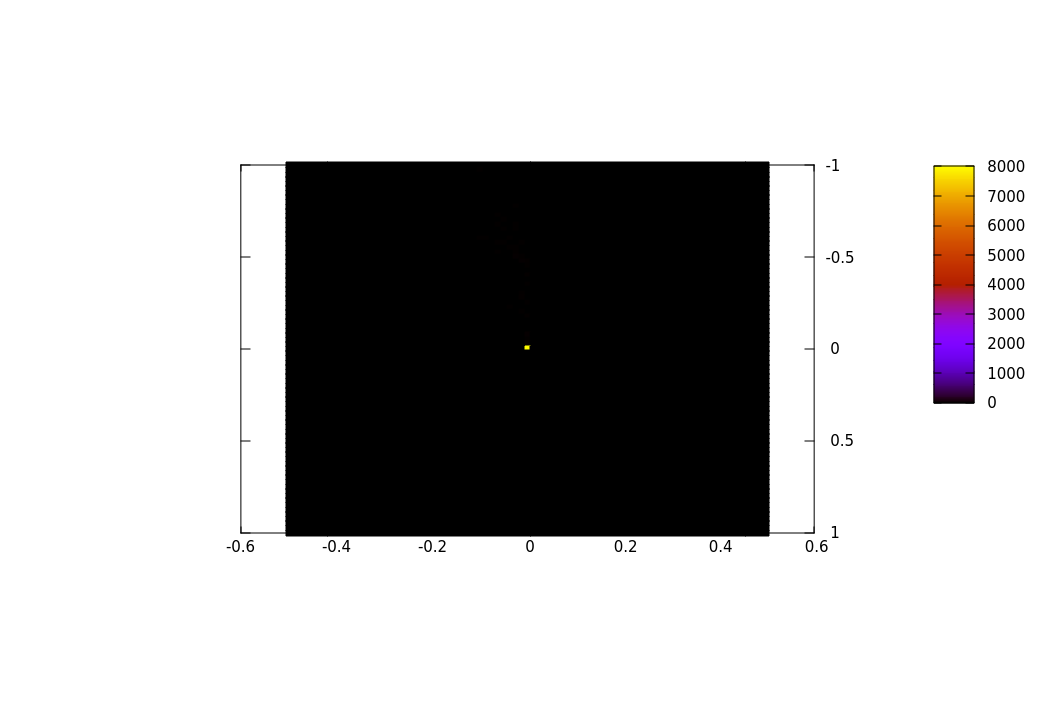
\includegraphics[width=0.6\textwidth]{picture9}
  \caption{для сетки \((80, 80)\)}
\end{figure}

\newpage
\subsection{Графики приближенного решения}
\noindent
\begin{figure}[ht!]
  \centering
  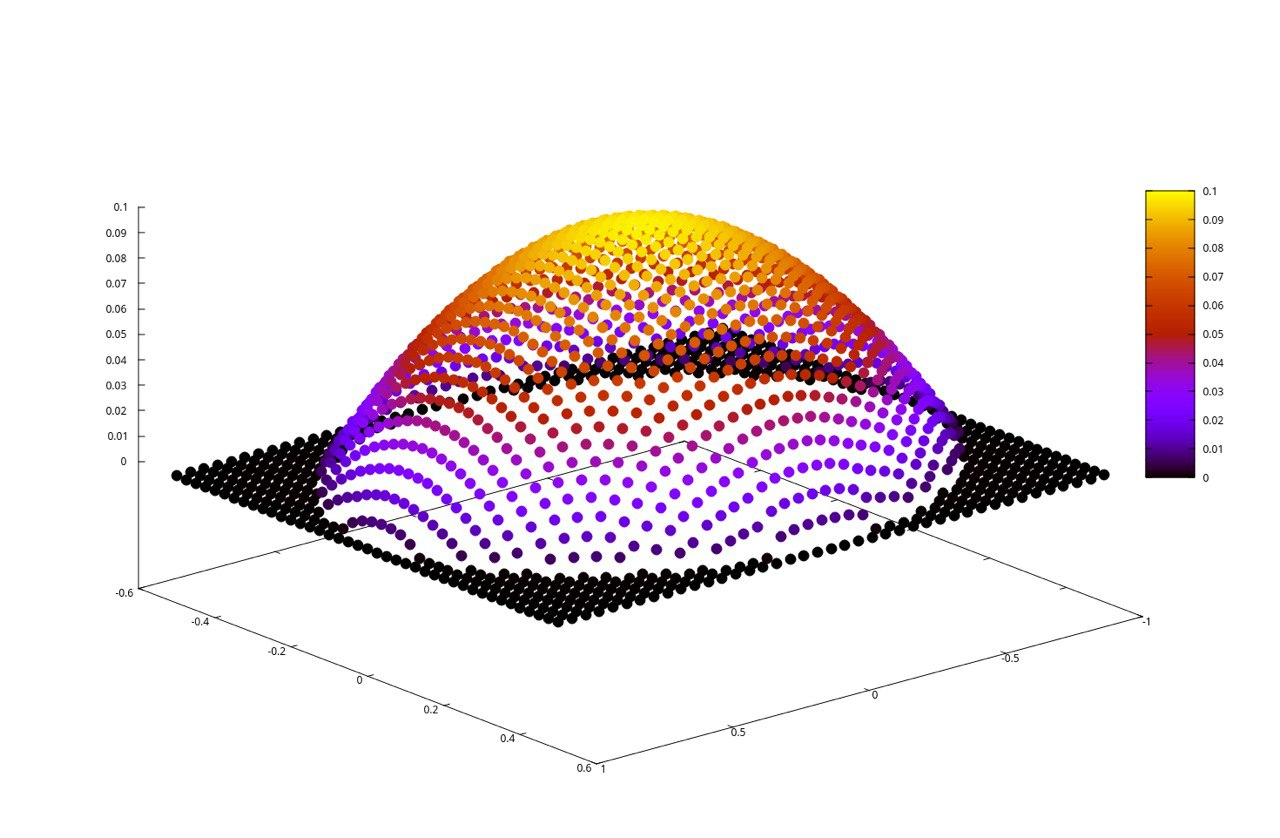
\includegraphics[width=0.90\textwidth]{picture1}
  \caption{График решения c сеткой \( 40 \times 40 \) точек}
\end{figure}

\begin{figure}[h!]
  \centering
  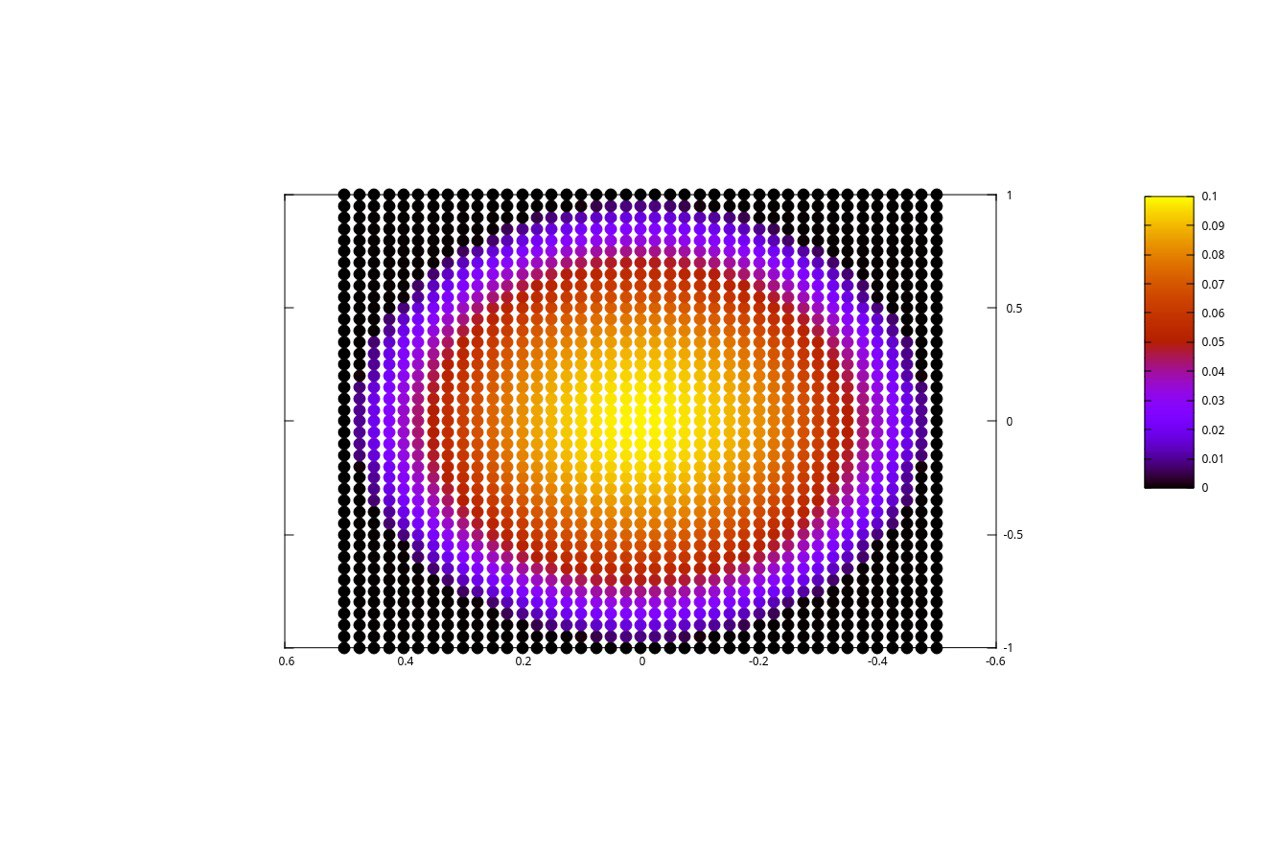
\includegraphics[width=0.65\textwidth]{picture2}
  \caption{Линии уровня с сеткой \( 40 \times 40 \) точек}
\end{figure}

\newpage
\noindent
\begin{figure}[h!]
  \centering
  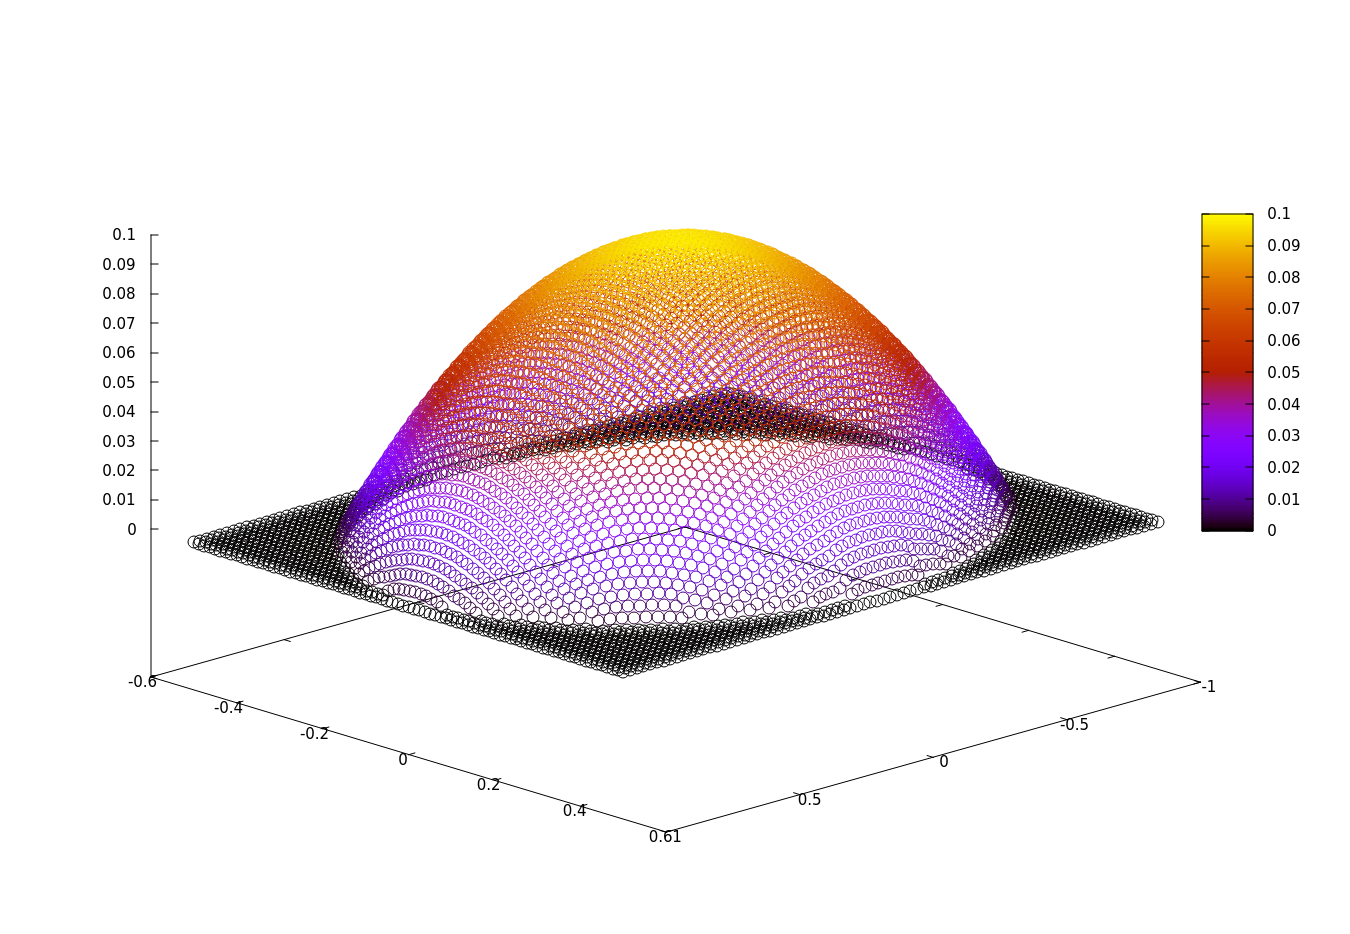
\includegraphics[width=1.0\textwidth]{picture3}
  \caption{График решения c сеткой \( 80 \times 80 \) точек}
\end{figure}

\begin{figure}[h!]
  \centering
  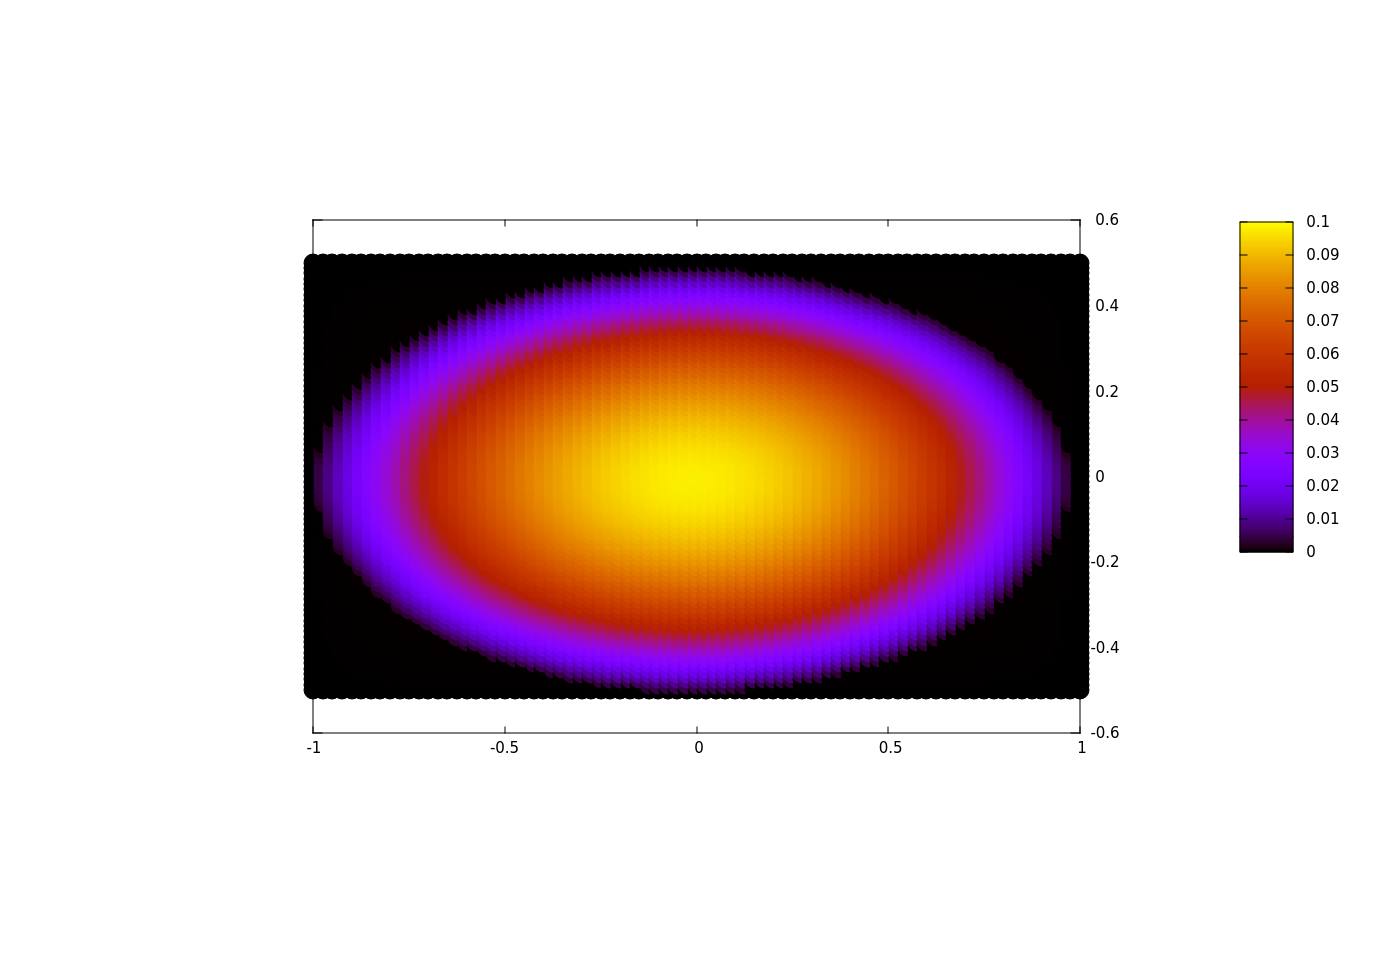
\includegraphics[width=0.65\textwidth]{picture4}
  \caption{Линии уровня c сеткой \( 80 \times 80 \) точек}
\end{figure}

\end{document}

